\section{Einf�hrung}

\subsection{Motivation}

\begin{frame}{\insertsubsection: Problem}
  \begin{block}<+->{Messger�te liefern unzuverl�ssige Daten}
    \begin{itemize}
      \item GPS Tracker sind nahe von Geb�uden unzuverl�ssig
      \item Sensoren sind empfindlich gegen�ber �u�ere Einfl�sse
          \begin{itemize}
              \item Z.B. starker Fall der Temperaturen bei einem Windzug
          \end{itemize}
    \end{itemize}
  \end{block}
\begin{figure}
    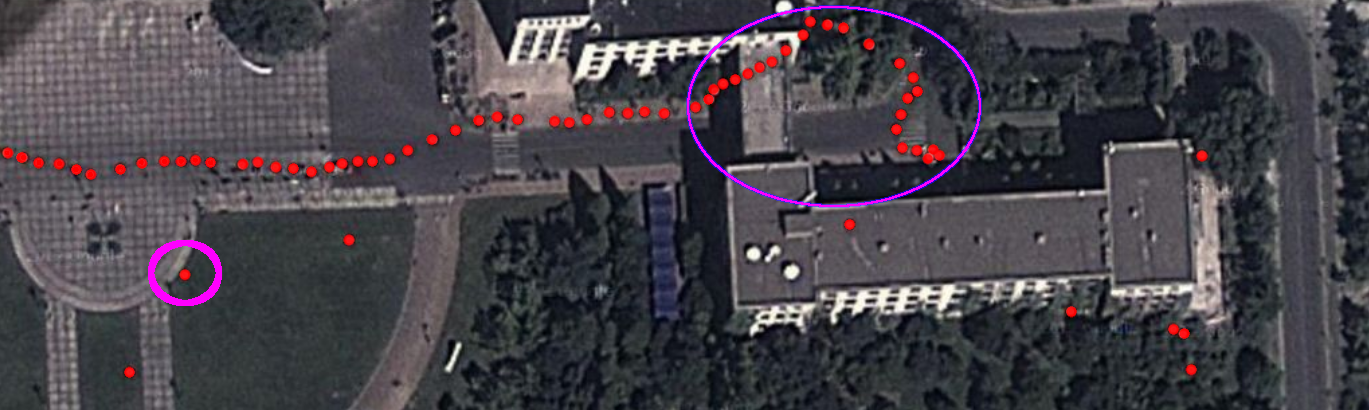
\includegraphics[width=\textwidth]{GPS_Motivation_Example.png}
    \caption{GPS-Tracking auf dem Campus der Tsinghua Universit�t \cite{Shaoxu17}}

\end{figure}

\end{frame}

\begin{frame}{\insertsubsection: Anwendungen der Anomalienerkennung}
  \begin{block}<+->{Umgang von unzuverl�ssigen Daten mit Anomalienerkennung}
    \begin{enumerate}
        \item Unzuverl�ssige Datenpunkte entfernen
            \begin{itemize}
                \item Ausrei�er werden entfernt  \smiley
                \item Entfernen aufeinanderfolgende Fehler machen Ergebnis unbrauchbar \textbf{oder}
                 werden als solche ggf. nicht entfernt \frownie
            \end{itemize}
        \item Unzuverl�ssige Datenpunkte reparieren
            \begin{itemize}
                \item Einzelne Ausrei�er werden leicht korrigiert \neutranie
                \item Aufeinanderfolgende Fehler werden zu stark ver�ndert (In der Praxis liegen die Messungen nahe bei den korrekten Werten) \neutranie
            \end{itemize}
    \end{enumerate}
  \end{block}
\end{frame}

\begin{frame}{\insertsubsection: Problemerweiterung}
    \begin{block}<+->{Hinzunahme von korrekt markierten Werten}
    \begin{enumerate}
        \item Markierung durch den Benutzer
            \begin{itemize}
            \item Z.B. markiert der Benutzer in beliebigen Zeitabst�nden seinen aktuellen Standort
            \end{itemize}
        \item Pr�zise Messger�te liefern in l�ngeren Zeitabst�nde korrekte Werte
    \end{enumerate}
  \end{block}
    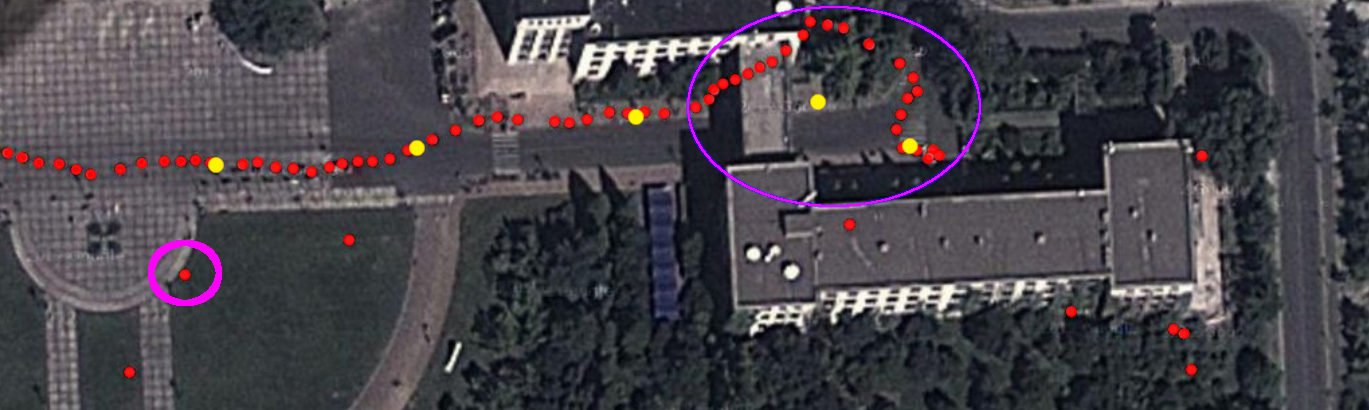
\includegraphics[width=\textwidth]{markierte_GPS_Motivation_Example.png}
\end{frame}



\subsection{Zielsetzung}

\begin{frame}{\insertsubsection}
  \begin{block}<+->{Ziel der Arbeit}
    \begin{enumerate}
      \item Ber�cksichtigung der markierten Werte in der Anomalienerkennung
            \begin{itemize}
                \item Aufeinanderfolgende Fehler sollen besser abgesch�tzt werden
            \end{itemize}
      \item Anomalienreparatur mit den Minimum-Change-Prinzip vereinbaren   
            \begin{itemize}
                \item Keine drastische Ver�nderungen der Messwerte
            \end{itemize}
        \item Neue Anomalienreparatur hinsichtlich Berechnungslaufzeit, Ergebnisgenauigkeit usw. optimieren
      \item Neue Anomalienreparatur mit unterschiedlichen Einstellungen  mit weitere Verfahren empirisch vergleichen
    \end{enumerate}
  \end{block}
\end{frame}


